\documentclass[conference]{IEEEtran}
\usepackage[utf8]{inputenc}
\usepackage{amsmath,amssymb}
\usepackage{graphicx}
\usepackage{booktabs}
\usepackage{hyperref}
\usepackage{url}
\usepackage{cite}
\usepackage{algorithm}
\usepackage{algorithmic}
\usepackage{multirow}
\usepackage{xcolor}
\usepackage{array}
\usepackage{tabularx}
\usepackage{makecell}

\graphicspath{{../src/figures/}}

\title{Graph Neural Networks for Advanced Persistent Threat Detection:\\A Scalable GraphSAGE Approach with Neighbour Sampling}

\author{
\IEEEauthorblockN{Manjunath Shivalingappa Javali}
\IEEEauthorblockA{Student ID: x24213896\\
H9AIMLC -- AI/ML in Cybersecurity\\
National College of Ireland\\
Dublin, Ireland\\
x24213896@student.ncirl.ie}
}

\begin{document}

\maketitle

% ─────────────────────────────────────────────────────────────────────────────
\begin{abstract}
Advanced Persistent Threats (APTs) employ multi-stage intrusion patterns and lateral movement that evade conventional rule-based detection. Traditional IDS analyse network events in isolation, failing to capture relational topology between hosts. This paper proposes a scalable GraphSAGE framework with neighbour sampling that enables graph-based APT detection on standard CPU hardware. We provide a formal graph-theoretic problem definition with complete message-passing equations and conduct a comparative evaluation across four model families---GraphSAGE, Random Forest, XGBoost, and MLP---on two benchmark datasets: CIC-IDS2017 (~2.8M flow records, 78 features) and ToN-IoT (~461K records). The two-layer GraphSAGE achieves F1 of 0.967 on CIC-IDS2017 and 0.954 on ToN-IoT, outperforming feature-only baselines while preserving inductive generalisation. Statistical validation across ten seeds confirms result stability (std$\leq$0.003).
\end{abstract}

\begin{IEEEkeywords}
Graph Neural Networks, Advanced Persistent Threats, GraphSAGE, Neighbour
Sampling, Network Intrusion Detection, CIC-IDS2017, ToN-IoT, Message Passing, Inductive Learning
\end{IEEEkeywords}

% ─────────────────────────────────────────────────────────────────────────────
\section{Introduction}

Advanced Persistent Threats (APTs) represent one of the most sophisticated
forms of cyberattack targeting organisations globally. Unlike opportunistic
malware or brute-force intrusions, APTs are distinguished by their multi-tiered
design, extended duration within compromised networks, and systematic use of
lateral movement techniques to achieve strategic objectives
\cite{gamage2025,hutchins2011}. Organisations frequently discover APT
intrusions months after initial compromise, during which time attackers
establish persistent footholds and exfiltrate sensitive data.

Traditional IDS exhibit fundamental limitations when confronting APTs.
Signature-based methods only detect previously documented attack patterns and
cannot identify novel or polymorphic threats \cite{bilot2024}. Anomaly-based
methods, while capable of detecting deviations from baseline behaviour, produce
unacceptably high false positive rates when faced with the ``low-and-slow''
characteristics typical of APT tactics. Critically, both paradigms analyse
individual network events in isolation, failing to capture the relationships
between hosts, processes, and communications that collectively define an APT
campaign.

Graph Neural Networks (GNNs) offer a theoretically compelling approach to this
detection challenge \cite{gilmer2017,xu2019gin}. By representing network
entities as nodes and their relationships as edges, GNNs enable multi-hop
reasoning and propagation of topological threat signals across the network graph
\cite{xu2024,zhou2020}. However, training full-graph GNNs on enterprise-scale
datasets poses considerable computational challenges, requiring substantial
memory and specialised hardware. Approaches such as FastGCN \cite{chen2018fastgcn} address this through
importance sampling of graph convolutions, yet this computational barrier has
created a significant gap between theoretical capability and operational utility.

This research addresses this gap through the following research question:
\textit{Can a GraphSAGE-based architecture employing neighbour sampling achieve
high-accuracy APT detection (F1-score $\geq 0.90$) from network flow data
whilst maintaining computational tractability for training on standard CPU-based
hardware?}

Two publicly available benchmark datasets are employed: CIC-IDS2017, comprising
approximately 2,830,743 network flow records with 78 features extracted by
CICFlowMeter (packet counts, inter-arrival times, flow duration, protocol
information), covering DoS/DDoS, brute-force, botnets, and infiltration based
on APT kill-chain patterns; and ToN-IoT, comprising approximately 461,043
records from a realistic IoT-enabled network environment with attack types
including Backdoor, DDoS, DoS, Injection, MITM, Password, Ransomware, Scanning,
and XSS. Both datasets provide per-flow feature vectors with binary labels
distinguishing normal (benign) from attack traffic. The key contributions of
this work are:

\begin{enumerate}
    \item A formal graph-theoretic problem definition for network-flow APT
    detection with rigorous message-passing equations.
    \item A scalable inductive GraphSAGE pipeline with neighbour sampling
    validated on CPU hardware (training time $<$\,0.5\,s).
    \item A comprehensive comparative evaluation including statistical
    significance testing, effect sizes, and confidence intervals across ten
    independent runs.
    \item An error analysis and threats-to-validity assessment that
    contextualise the performance ceiling observed on benchmark datasets.
    \item An expanded ethics discussion encompassing GDPR Article~22, the EU
    AI Act, adversarial robustness, and dual-use considerations.
\end{enumerate}

% ─────────────────────────────────────────────────────────────────────────────
\section{Related Work}

\subsection{Foundational Graph Neural Network Architectures}

Kipf and Welling \cite{kipf2017} introduced Graph Convolutional Networks
(GCNs), which generalise spectral convolutions to irregular graph domains via a
first-order Chebyshev approximation of the graph Laplacian, achieving
state-of-the-art semi-supervised node classification on citation graphs.
\textbf{Key finding:} GCNs achieve over 81\% accuracy on the Cora citation
benchmark, substantially outperforming spectral competitors.
\textbf{Limitation:} The architecture is inherently transductive, requiring the
full adjacency matrix at training time, which precludes application to
dynamically evolving network graphs where new hosts and flows appear
continuously. \textbf{This work addresses} the transductive limitation by
adopting the inductive GraphSAGE framework \cite{hamilton2017}, which learns
transferable aggregation functions rather than fixed node embeddings.

Hamilton, Ying and Leskovec \cite{hamilton2017} proposed GraphSAGE, which
replaces the full-graph spectral convolution with a sample-and-aggregate
strategy that learns neighbourhood aggregation functions from sampled subsets of
each node's local neighbourhood. GraphSAGE has since been applied successfully
beyond its original social-network setting, including large-scale recommendation
systems \cite{ying2018graphsage_rec}. \textbf{Key finding:} GraphSAGE achieves
superior accuracy on the Reddit and PPI datasets while reducing memory
consumption by orders of magnitude relative to full-graph methods.
\textbf{Limitation:} The original evaluation focused on social-network and
biological datasets, leaving efficacy on cybersecurity graph structures largely
unexplored. \textbf{This work addresses} this gap by evaluating GraphSAGE on
network-flow graphs constructed from CIC-IDS2017 and ToN-IoT benchmark data.

Veli\v{c}kovi\'{c} et al.~\cite{velickovic2018} introduced Graph Attention
Networks (GATs), which replace fixed neighbourhood aggregation weights with a
learned attention mechanism, enabling the model to assign varying importance to
different neighbours. \textbf{Key finding:} GATs improve node classification
accuracy over GCNs by 1.5\% on the Citeseer benchmark.
\textbf{Limitation:} Quadratic attention computation over large neighbourhoods
introduces substantial memory overhead, making unmodified GATs impractical for
enterprise-scale network graphs. \textbf{This work addresses} this concern by
employing mean aggregation with neighbour sampling, reducing memory complexity
from $O(|\mathcal{V}|^2)$ to $O(B \cdot \prod_l S_l)$.

Xu et al.~\cite{xu2019gin} proved that Graph Isomorphism Networks (GIN), using
a sum aggregator, are as expressive as the Weisfeiler-Lehman graph isomorphism
test, establishing a formal upper bound on GNN discriminative power.
\textbf{Key finding:} Mean and max aggregators are strictly less powerful than
sum aggregators for distinguishing graph structures. \textbf{Limitation:}
Theoretical expressiveness does not directly translate to superior empirical
performance in noisy real-world datasets. \textbf{This work addresses} this
observation by empirically comparing GNN layer counts rather than aggregation
functions, isolating the depth--performance trade-off.

Gilmer et al.~\cite{gilmer2017} unified GNN variants under the Message Passing
Neural Network (MPNN) framework, showing that GCN, GGNN, and SchNet are all
special cases of a general message--aggregate--update paradigm.
\textbf{Key finding:} MPNN achieves near-chemical-accuracy on quantum chemistry
property prediction benchmarks, demonstrating the generality of the framework.
\textbf{Limitation:} The MPNN formulation was designed for molecular property
prediction and does not address scalability to large sparse graphs typical of
network security. \textbf{This work positions} GraphSAGE as a scalable
instantiation of the MPNN framework applied to network security.

\subsection{Classical Intrusion Detection and Anomaly Detection}

Paxson \cite{paxson1999} pioneered network-level intrusion detection with the
Bro (now Zeek) system, performing real-time protocol analysis and pattern
matching on packet streams. \textbf{Key finding:} Bro can detect a wide variety
of intrusion scenarios with low false positive rates when attack signatures are
known. \textbf{Limitation:} Reliance on handcrafted rules limits detection of
novel attack vectors, and the system operates on individual connection records
without modelling inter-host relationships. \textbf{This work addresses} this
by replacing rule-based detection with a learned graph representation.

Chandola, Banerjee and Kumar \cite{chandola2009} presented an authoritative
survey of anomaly detection spanning statistical, classification-based,
clustering, and information-theoretic paradigms. \textbf{Key finding:}
Unsupervised methods detect unknown attack patterns but suffer from high false
positive rates; supervised approaches require expensive labelled data.
\textbf{Limitation:} Neither paradigm captures relational structure between
network entities. \textbf{This work addresses} this by combining supervised
classification with graph-structural features.

Buczak and Guven \cite{buczak2016} surveyed machine learning methods for
intrusion detection, evaluating decision trees, random forests, SVMs, and neural
networks on benchmark datasets. \textbf{Key finding:} Ensemble methods
consistently achieve strong baseline performance on tabular flow features but
discard relational information. \textbf{Limitation:} All evaluated methods
treat each flow independently. \textbf{This work addresses} this by including
Random Forest and XGBoost as competitive baselines while adding graph topology
through GNN message passing.

\subsection{APT Lifecycle Frameworks and Threat Modelling}

Hutchins, Cloppert and Amin \cite{hutchins2011} formalised the Cyber Kill Chain
model, decomposing APT campaigns into seven sequential phases from
reconnaissance through actions on objectives. \textbf{Key finding:} The
kill-chain model provides a structured vocabulary for describing APT campaigns
and guides defensive countermeasures. \textbf{Limitation:} The linear model
oversimplifies modern APT campaigns, which frequently exhibit non-linear,
iterative behaviour. \textbf{This work addresses} this by modelling APT
detection as graph classification, which captures concurrent multi-stage
patterns without imposing sequential structure.

Strom et al.~\cite{strom2018} developed the MITRE ATT\&CK framework, a
knowledge base of adversary tactics, techniques, and procedures (TTPs) derived
from real-world observations. \textbf{Key finding:} ATT\&CK provides more
granular and flexible vocabulary than the kill chain, enabling systematic
evaluation of detector coverage. \textbf{Limitation:} ATT\&CK does not
prescribe detection methods, leaving the mapping from detectors to TTP coverage
under-explored. \textbf{This work acknowledges} this limitation as a direction
for future work.

\subsection{GNN-Based Malware and Threat Detection}

Iorizzo and Yuan \cite{iorizzo2024} demonstrated 98\% classification accuracy
using GNNs with Ghidra P-Code for malware detection across multiple binary
architectures. \textbf{Key finding:} Control-flow graph representations of
binaries are highly discriminative for malware family classification.
\textbf{Limitation:} The approach is limited to static binary analysis and
cannot detect APT activity in runtime network traffic. \textbf{This work
addresses} this by targeting runtime network flow data.

Bilot et al.~\cite{bilot2024} conducted an extensive survey of graph
representation learning approaches for malware detection, concluding that
GNN-based techniques generally outperform traditional machine learning methods.
\textbf{Key finding:} GNN-based approaches improve detection rates by up to
15\% over feature-only classifiers on binary malware datasets.
\textbf{Limitation:} Poor generalisation across datasets and vulnerability to
overfitting persist as challenges. \textbf{This work addresses} this through
neighbour sampling and evaluation across multiple datasets with seed sensitivity
analysis.

Liu et al.~\cite{liu2018} proposed Log2vec, which constructs heterogeneous
graphs from enterprise audit logs and applies graph embedding to detect malicious
activity. \textbf{Key finding:} Heterogeneous graph embeddings capture semantic
relationships among diverse event types more effectively than homogeneous
approaches. \textbf{Limitation:} Substantial domain expertise is required to
define the heterogeneous schema, and evaluation was limited to a single
enterprise environment. \textbf{This work addresses} this by adopting
homogeneous flow-level graphs that generalise across organisations without
schema customisation.

\subsection{Provenance Graph and APT Detection}

Xu et al.~\cite{xu2024} proposed ProcSAGE, a GraphSAGE variant converting
system call audit logs into provenance graphs, achieving over 95\% accuracy with
inductive learning. \textbf{Key finding:} Inductive GNN methods outperform
transductive variants for host-based threat detection by enabling
generalisation to unseen processes. \textbf{Limitation:} Evaluation was limited
to single-host audit logs without cross-host lateral movement detection, and
synthetic datasets precluded enterprise-level validation. \textbf{This work
addresses} this by operating at the network flow level, capturing cross-host
communication patterns.

Ren et al.~\cite{ren2023} employed GCNs on provenance graphs from real APT
campaigns, achieving 90--92\% accuracy. \textbf{Key finding:} GCN-based
detection outperforms feature-only baselines on real APT campaign data.
\textbf{Limitation:} GCNs are inherently transductive, requiring the complete
graph during training. \textbf{This work addresses} this by adopting the
inductive GraphSAGE architecture, which classifies unseen nodes without
retraining.

Wang et al.~\cite{wang2025} integrated graph attention networks with temporal
modelling for APT detection in edge computing environments. \textbf{Key
finding:} Temporal graph attention improves detection of progressive attack
stages by 3--5\% over static GCN baselines. \textbf{Limitation:} The absence
of comparison with traditional IDS baselines reduces reproducibility, and
inference latency across distributed systems remains uncharacterised.
\textbf{This work addresses} reproducibility concerns by providing explicit
baseline comparisons and training-time measurements.

King and Chen \cite{king2003} introduced backtracking as a provenance-based
intrusion analysis technique, enabling analysts to trace causal dependencies
from a detected intrusion backward through the system-event chain.
\textbf{Key finding:} Provenance graphs enable forensic root-cause analysis
unavailable to event-level detectors. \textbf{Limitation:} The dependency
explosion problem causes long-running processes to accumulate so many causal
edges that graphs become intractable without pruning. \textbf{This work
addresses} this via neighbour sampling, which bounds subgraph size during
training.

Han et al.~\cite{han2020} proposed Unicorn, a runtime APT detector that
constructs streaming provenance graphs from system audit logs and applies graph
sketching to build fixed-size histogram representations. \textbf{Key finding:}
Unicorn achieves high detection rates with low false positive rates on DARPA TC
dataset APT scenarios, processing provenance graphs in near real-time.
\textbf{Limitation:} Histogram summarisation sacrifices fine-grained structural
information that GNN-based approaches can exploit, and threshold tuning may not
transfer across environments. \textbf{This work addresses} this by retaining
full structural information through learned GNN representations.

\subsection{Hybrid and Alternative Approaches}

Xuan and Nguyen \cite{xuan2024} proposed a hybrid CNN-RNN framework for APT
detection on public datasets. \textbf{Key finding:} Temporal features improve
accuracy over static approaches by capturing sequential attack patterns.
\textbf{Limitation:} The absence of graph-based representations results in loss
of topological relationship data required for identifying multi-hop propagation
paths. \textbf{This work addresses} this by incorporating explicit graph
topology through GNN message passing.

Mead and Arabo \cite{mead2025} utilised heterogeneous GNNs with threat
intelligence feeds for APT attribution. \textbf{Key finding:} Heterogeneous
GNNs improve attribution accuracy by leveraging diverse node types (IP, domain,
hash). \textbf{Limitation:} Focus on attribution rather than real-time
detection introduces time delays incompatible with threat response.
\textbf{This work addresses} this by targeting real-time network flow
classification rather than post-hoc attribution.

Gamage, Gutierrez and Ray \cite{gamage2025} provided a comprehensive systematic
literature review identifying scalability as the most significant unresolved
challenge facing GNN-based threat detection. \textbf{Key finding:} Most GNN
detection systems are evaluated only against limited static graphs without
enterprise-level validation. \textbf{Limitation:} The review does not propose
a solution; scalability remains open. \textbf{This work directly addresses}
this gap by demonstrating CPU-tractable training via neighbour sampling.

\subsection{Related Work Summary and Research Gap}

Table~\ref{tab:related_work} summarises the key related works and positions the
present study within the literature. The synthesis reveals that no existing work
has achieved a scalable, inductive framework evaluated against standardised
\textit{network flow} benchmarks while maintaining CPU-based computational
tractability. Provenance-graph approaches \cite{xu2024,ren2023,han2020,king2003}
operate at the system-call level on individual hosts, whereas network-flow-level
detection requires cross-host graph construction that preserves communication
topology. This study addresses the gap by combining GraphSAGE's inductive
generalisation with neighbour sampling on CIC-IDS2017 and ToN-IoT, with
explicit baseline comparisons to quantify the marginal contribution of graph
structure.

\begin{table*}[t]
\centering
\caption{Summary of Key Related Works in GNN-Based and Graph-Assisted Threat Detection}
\label{tab:related_work}
\renewcommand{\arraystretch}{1.25}
\begin{tabular}{p{2.8cm} p{3.4cm} p{2.6cm} p{2.4cm} p{4.2cm}}
\toprule
\textbf{Author / Year} & \textbf{Method} & \textbf{Dataset} & \textbf{Key Metric} & \textbf{Primary Limitation} \\
\midrule
Kipf \& Welling \cite{kipf2017} (2017) & Graph Convolutional Network (GCN) & Cora, Citeseer, Pubmed & Acc: 81.5\% & Transductive; cannot classify unseen nodes \\
Hamilton et al.\ \cite{hamilton2017} (2017) & GraphSAGE; sampled neighbourhood aggregation & Reddit, PPI, Citation & F1: 0.950 & Evaluated only on social/biological graphs; no cybersecurity application \\
Veli\v{c}kovi\'{c} et al.\ \cite{velickovic2018} (2018) & Graph Attention Network (GAT) & Cora, Citeseer, PPI & Acc: 83.0\% & Quadratic attention memory; impractical for large enterprise graphs \\
Xu et al.\ \cite{xu2019gin} (2019) & Graph Isomorphism Network (GIN); sum aggregation & Bioinformatics, social & Acc: 89.4\% & Higher expressiveness does not guarantee real-world gains; no security datasets \\
Han et al.\ \cite{han2020} (2020) & Unicorn; streaming provenance + graph sketching & DARPA TC & DR: $>$95\% & Histogram representation discards fine-grained structure; threshold sensitivity \\
Liu et al.\ \cite{liu2018} (2019) & Log2vec; heterogeneous graph embedding & Enterprise audit logs & AUC: 0.99 & Requires custom schema; single-enterprise validation only \\
Ren et al.\ \cite{ren2023} (2023) & GCN on provenance graphs & Real APT campaigns & Acc: 90--92\% & Transductive GCN; poor scalability to new nodes \\
Xu et al.\ \cite{xu2024} (2024) & ProcSAGE; inductive GraphSAGE on audit logs & Synthetic host logs & Acc: $>$95\% & Single-host only; no cross-host lateral movement; synthetic data only \\
Xuan \& Nguyen \cite{xuan2024} (2024) & Hybrid CNN-RNN on flow features & CICIDS, UNSW-NB15 & F1: 0.97 & No graph topology; cannot capture multi-hop propagation \\
\textbf{This Work} (2025) & \textbf{GraphSAGE + neighbour sampling on flow graphs} & \textbf{CIC-IDS2017, ToN-IoT} & \textbf{F1: 0.967} & \textbf{Benchmark data; offline evaluation} \\
\bottomrule
\end{tabular}
\end{table*}

% ─────────────────────────────────────────────────────────────────────────────
\section{Problem Definition}

\subsection{Formal Problem Statement}

Let a network communication graph be defined as $G = (V, E, X)$, where:
\begin{itemize}
    \item $V = \{v_1, v_2, \ldots, v_n\}$ is the set of $n$ nodes, each
    representing a network flow record;
    \item $E \subseteq V \times V$ is the set of edges, where $(v_i, v_j) \in E$
    if flows $v_i$ and $v_j$ share a common source or destination IP address,
    encoding the topological communication relationship between network entities;
    \item $X \in \mathbb{R}^{|V| \times d}$ is the node feature matrix, where
    each row $\mathbf{x}_v \in \mathbb{R}^d$ encodes the $d$-dimensional
    statistical flow features (packet counts, byte volumes, inter-arrival
    statistics, flag counts, etc.) of node $v$.
\end{itemize}

The binary classification objective is to learn a parametric function:
\begin{equation}
f_\theta: G \rightarrow \{0, 1\}^{|V|}
\label{eq:problem}
\end{equation}
where $f_\theta(v) = 1$ denotes a malicious (APT-related) flow and
$f_\theta(v) = 0$ denotes a benign flow, and $\theta$ are the learned model
parameters. Because new flows continuously arrive in operational networks,
the function $f_\theta$ must be \textit{inductive}: it must classify previously
unseen nodes without retraining, using only the local neighbourhood
$\mathcal{N}(v)$ and feature vector $\mathbf{x}_v$.

\subsection{Graph Construction Formalisation}

Given a raw dataset of flow records $\mathcal{D} = \{(r_i, y_i)\}_{i=1}^N$,
where $r_i$ denotes the feature vector of the $i$-th flow and
$y_i \in \{0, 1\}$ its binary label, the graph construction proceeds as:

\begin{equation}
E = \left\{(i, j) \mid \text{IP}^{src}_i = \text{IP}^{src}_j \lor
\text{IP}^{dst}_i = \text{IP}^{dst}_j,\ i \neq j \right\}
\end{equation}

To prevent degree explosion from high-traffic hosts (hub nodes), each node's
degree is capped at $K = 10$ neighbours, selected uniformly at random:
\begin{equation}
\mathcal{N}_{\text{cap}}(v) = \text{SAMPLE}\bigl(\mathcal{N}(v),
\min(|\mathcal{N}(v)|, K)\bigr)
\end{equation}

% ─────────────────────────────────────────────────────────────────────────────
\section{Methodology and Implementation}

\subsection{Dataset Description}

Two benchmark datasets are employed for evaluation, both providing per-flow
feature vectors (packet counts, inter-arrival times, flow duration, protocol
information) suitable for graph-based analysis.

\textbf{CIC-IDS2017}~\cite{sharafaldin2018} is the primary dataset, comprising
2,830,743 network flow records with 78 features extracted by the CICFlowMeter
tool. The dataset covers attack types aligned with APT kill-chain patterns:
Benign, DoS Hulk, PortScan, DDoS, DoS GoldenEye, FTP-Patator, SSH-Patator,
DoS Slowloris, DoS Slowhttptest, Bot, Web Attack, Infiltration, and Heartbleed.
Labels are binarised into two classes: \textit{Benign} and \textit{Attack}.

\textbf{ToN-IoT}~\cite{alsaedi2020} is a complementary dataset based on a realistic IoT-enabled
business network environment, comprising 461,043 records. Attack types include
Backdoor, DDoS, DoS, Injection, MITM, Password, Ransomware, Scanning, and XSS.
Labels are binarised into \textit{Normal} and \textit{Attack} for binary
classification.

\subsection{Dataset Validation and Representativeness}

CIC-IDS2017~\cite{sharafaldin2018} is one of the most widely adopted modern
benchmarks for network intrusion detection, superseding the earlier NSL-KDD
dataset \cite{tavallaee2009}, and was generated by the Canadian Institute
for Cybersecurity using realistic network traffic profiles and attack scenarios.
ToN-IoT provides complementary evaluation in an IoT-specific threat landscape.
Together, these datasets enable comprehensive evaluation across diverse network
environments.

The datasets provide four concrete advantages for this study:
(a)~\textbf{reproducibility}---both datasets are publicly available, ensuring
any researcher can replicate reported results;
(b)~\textbf{known ground truth labels}---CIC-IDS2017 attack labels are assigned
by matching traffic to known attack time windows, and ToN-IoT labels are
generated from controlled attack execution in a testbed environment;
(c)~\textbf{rich feature sets}---CIC-IDS2017 provides 78 CICFlowMeter features
capturing flow-level, packet-level, and inter-arrival statistics suitable for
graph-based analysis; and (d)~\textbf{scale}---approximately 2.8M records
(CIC-IDS2017) and 461K records (ToN-IoT) provide sufficient volume to evaluate
graph construction and neighbour sampling at non-trivial scale.

For CIC-IDS2017, the class balance after binarisation yields approximately
83\% benign and 17\% attack records. For ToN-IoT, approximately 30\% of
records are normal and 70\% are attack traffic.

While benchmark data cannot capture all production-environment complexities
such as concept drift and adversarial evasion, it enables controlled
ablation studies impossible with operational data where confounding variables
cannot be isolated.

\subsection{Data Preprocessing}

The preprocessing pipeline comprises six steps:
\begin{enumerate}
    \item Removal of rows containing NaN or infinite-valued features.
    \item One-hot encoding of categorical features (e.g., protocol type,
    service flags), expanding the feature space accordingly.
    \item Binary label encoding: benign/normal$\,=\,0$, attack$\,=\,1$.
    \item Z-score normalisation using \texttt{StandardScaler} applied
    \textit{fit-only} on the training split to prevent data leakage.
    \item Stratified train/validation/test splitting (70\%/15\%/15\%) to
    preserve class distribution across all folds.
    \item Graph construction from the processed features (see below).
\end{enumerate}

\subsection{Graph Construction}

Network flows are modelled as a communication graph where each flow constitutes
a node with its feature vector as node attributes. Edges connect flows sharing
common source or destination IP addresses, capturing the topological
relationships between network entities that characterise multi-stage attack
campaigns. For CIC-IDS2017 and ToN-IoT, source and destination IP addresses
are extracted from the flow records. Neighbour connections are limited to
$K = 10$ per IP address to prevent memory explosion from hub nodes.

\subsection{GraphSAGE Message Passing Equations}

The GraphSAGE architecture \cite{hamilton2017} implements three operations per
layer, constituting a Message Passing Neural Network \cite{gilmer2017}:

\textbf{(1) Neighbourhood Aggregation:}
\begin{equation}
\mathbf{h}_{\mathcal{N}(v)}^{(l)} = \text{AGGREGATE}^{(l)}\!\left(\left\{
\mathbf{h}_u^{(l-1)} \;\middle|\; \forall u \in \mathcal{N}(v)\right\}\right)
\label{eq:aggregate}
\end{equation}
In this work, $\text{AGGREGATE}$ is the element-wise mean:
\begin{equation}
\text{AGGREGATE}^{(l)}_{\text{mean}}\!\left(\mathcal{S}\right)
= \frac{1}{|\mathcal{S}|} \sum_{\mathbf{h} \in \mathcal{S}} \mathbf{h}
\label{eq:mean_agg}
\end{equation}

\textbf{(2) Node Embedding Update:}
\begin{equation}
\mathbf{h}_v^{(l)} = \sigma\!\left(\mathbf{W}^{(l)} \cdot
\left[\mathbf{h}_v^{(l-1)} \,\|\, \mathbf{h}_{\mathcal{N}(v)}^{(l)}\right]
+ \mathbf{b}^{(l)}\right)
\label{eq:update}
\end{equation}
where $\mathbf{W}^{(l)} \in \mathbb{R}^{d_l \times 2d_{l-1}}$ and
$\mathbf{b}^{(l)} \in \mathbb{R}^{d_l}$ are learnable parameters,
$[\,\cdot\,\|\,\cdot\,]$ denotes concatenation, and $\sigma(\cdot)$ is the
ReLU activation function. Initial embeddings are set to the raw features:
$\mathbf{h}_v^{(0)} = \mathbf{x}_v$.

\textbf{(3) $\ell_2$ Normalisation:}
\begin{equation}
\mathbf{h}_v^{(l)} \leftarrow
\frac{\mathbf{h}_v^{(l)}}{\max\!\left(\left\|\mathbf{h}_v^{(l)}\right\|_2,
\epsilon\right)}
\label{eq:normalise}
\end{equation}

\textbf{(4) Graph Readout (node-level classification):}

For node-level classification, the final-layer embedding is passed directly to
a linear classifier without a global pooling step:
\begin{equation}
\hat{y}_v = \text{softmax}\!\left(\mathbf{W}_c \cdot \mathbf{h}_v^{(L)}
+ \mathbf{b}_c\right)
\label{eq:readout}
\end{equation}
where $L$ is the total number of GraphSAGE layers and
$\mathbf{W}_c, \mathbf{b}_c$ are the classification head parameters.

\subsection{Neighbour Sampling for Scalability}

During training, mini-batches are constructed using ancestral sampling: given a
batch of target nodes, their first-hop neighbours are sampled (up to $S_1 = 15$)
and their second-hop neighbours are sampled (up to $S_2 = 10$). This reduces
memory complexity from $O(|V|)$ to $O(B \cdot S_1 \cdot S_2)$, where $B$ is
the batch size, enabling scalable training without loading the entire graph
adjacency matrix into memory.

\subsection{Baseline Models}

Three feature-only baselines are implemented for comparison:
\begin{itemize}
    \item \textbf{Random Forest (RF)}: 200 estimators, max depth 20, Gini
    impurity criterion. Operates exclusively on node feature vectors.
    \item \textbf{XGBoost}: 200 estimators, max depth 8, learning rate 0.1,
    subsampling 0.8, column subsampling 0.8.
    \item \textbf{MLP}: Two hidden layers (128 neurons, 64 neurons), ReLU
    activations, dropout 0.3, early stopping with patience 10 on validation
    F1-score.
\end{itemize}

These baselines operate on node features without graph structure, enabling
direct assessment of whether topological information provides detection
advantages beyond feature-level signals.

\subsection{Training Configuration}

All models are trained exclusively on CPU hardware to validate the research
question regarding computational tractability. Full hyperparameter
specifications are provided in Table~\ref{tab:hyperparams}.

\begin{table}[htbp]
\centering
\caption{Complete Hyperparameter Specifications for All Models}
\label{tab:hyperparams}
\renewcommand{\arraystretch}{1.2}
\begin{tabular}{lll}
\toprule
\textbf{Hyperparameter} & \textbf{GraphSAGE 2L} & \textbf{GraphSAGE 3L} \\
\midrule
Learning rate & 0.01 & 0.01 \\
Optimiser & Adam & Adam \\
Weight decay & $5 \times 10^{-4}$ & $5 \times 10^{-4}$ \\
Epochs (max) & 200 & 200 \\
Early stopping patience & 15 & 15 \\
Batch size & 512 & 512 \\
Hidden dimensions & 64 & 64 \\
Output dimension & 2 & 2 \\
Number of GNN layers & 2 & 3 \\
Aggregation function & Mean & Mean \\
Dropout rate & 0.0 & 0.0 \\
1st-hop sample size $S_1$ & 15 & 15 \\
2nd-hop sample size $S_2$ & 10 & 10 \\
3rd-hop sample size $S_3$ & --- & 5 \\
Loss function & Cross-entropy & Cross-entropy \\
\midrule
\textbf{Hyperparameter} & \textbf{RF} & \textbf{XGBoost} \\
\midrule
Number of estimators & 200 & 200 \\
Max depth & 20 & 8 \\
Learning rate & --- & 0.1 \\
Criterion & Gini & --- \\
Subsample & --- & 0.8 \\
Col. subsample & --- & 0.8 \\
Min samples leaf & 1 & --- \\
\midrule
\textbf{Hyperparameter} & \multicolumn{2}{l}{\textbf{MLP}} \\
\midrule
Hidden layers & \multicolumn{2}{l}{[128, 64]} \\
Activation & \multicolumn{2}{l}{ReLU} \\
Dropout rate & \multicolumn{2}{l}{0.3} \\
Optimiser & \multicolumn{2}{l}{Adam, lr=0.001} \\
Early stopping patience & \multicolumn{2}{l}{10} \\
\bottomrule
\end{tabular}
\end{table}

\subsection{Computational Complexity Analysis}

\textbf{GraphSAGE} with $L$ layers, $|E|$ edges, and embedding dimension $d$
has per-epoch time complexity of $O(L \cdot |E| \cdot d)$ for full-graph
inference. With neighbour sampling, this reduces to $O(B \cdot S_1 \cdot S_2
\cdot d)$ per mini-batch, where $B$ is batch size---a constant independent of
$|E|$, enabling linear scaling in dataset size.

\textbf{Random Forest} with $T$ trees, $n$ training samples, and $m$ features
has training complexity $O(T \cdot m \cdot n \log n)$. Prediction complexity
is $O(T \cdot \log n)$ per sample, making inference highly efficient.

\textbf{XGBoost} adds $T$ trees sequentially with complexity $O(T \cdot n
\cdot d \cdot \log n)$ per iteration under histogram-based splitting
\cite{chen2016xgboost}, which in practice is faster than Random Forest due to
the more aggressive subsampling.

\textbf{MLP} with two hidden layers of width $h$ has training complexity
$O(n \cdot d \cdot h)$ per epoch, which scales linearly with dataset size but
without the structural information that graph-based models extract.

In practice, as reported in Table~\ref{tab:results}, XGBoost is fastest on
these datasets owing to its aggressive subsampling, followed by MLP, RF, and
GraphSAGE 2L. The overhead of GraphSAGE relative to XGBoost is attributable to
the neighbour-sampling and message-passing steps absent from feature-only
models.

% ─────────────────────────────────────────────────────────────────────────────
\section{Evaluation}

\subsection{Performance Metrics}

The following metrics are employed:
\begin{itemize}
    \item \textbf{F1-Score} (primary metric): Harmonic mean of precision and
    recall, appropriate for class-imbalanced network data. Threshold: $\geq 0.90$.
    \item \textbf{Accuracy}: Overall classification correctness.
    \item \textbf{Precision}: Proportion of true positives among predicted
    positives (minimising false alert burden).
    \item \textbf{Recall}: Proportion of true positives correctly identified
    (minimising missed detections).
    \item \textbf{AUC-ROC}: Threshold-independent discriminative capability.
    \item \textbf{Training Time}: Wall-clock seconds on CPU for tractability
    assessment.
\end{itemize}

\subsection{Results}

All reported metrics include $\pm$ standard deviation error bands computed
over 10 seeds (seeds 0--9). Figures~\ref{fig:model_comparison} and
\ref{fig:training_time} display error bars representing one standard deviation
across 10 random initialisations, enabling visual assessment of result
stability.

\begin{figure}[htbp]
\centering

\includegraphics[width=\columnwidth]{training_curves_2layer.png}
\caption{Training and validation loss/F1-score curves for the 2-layer
GraphSAGE model across epochs, illustrating rapid convergence within 10 epochs.}
\label{fig:training_curves}
\end{figure}

\begin{figure}[htbp]
\centering
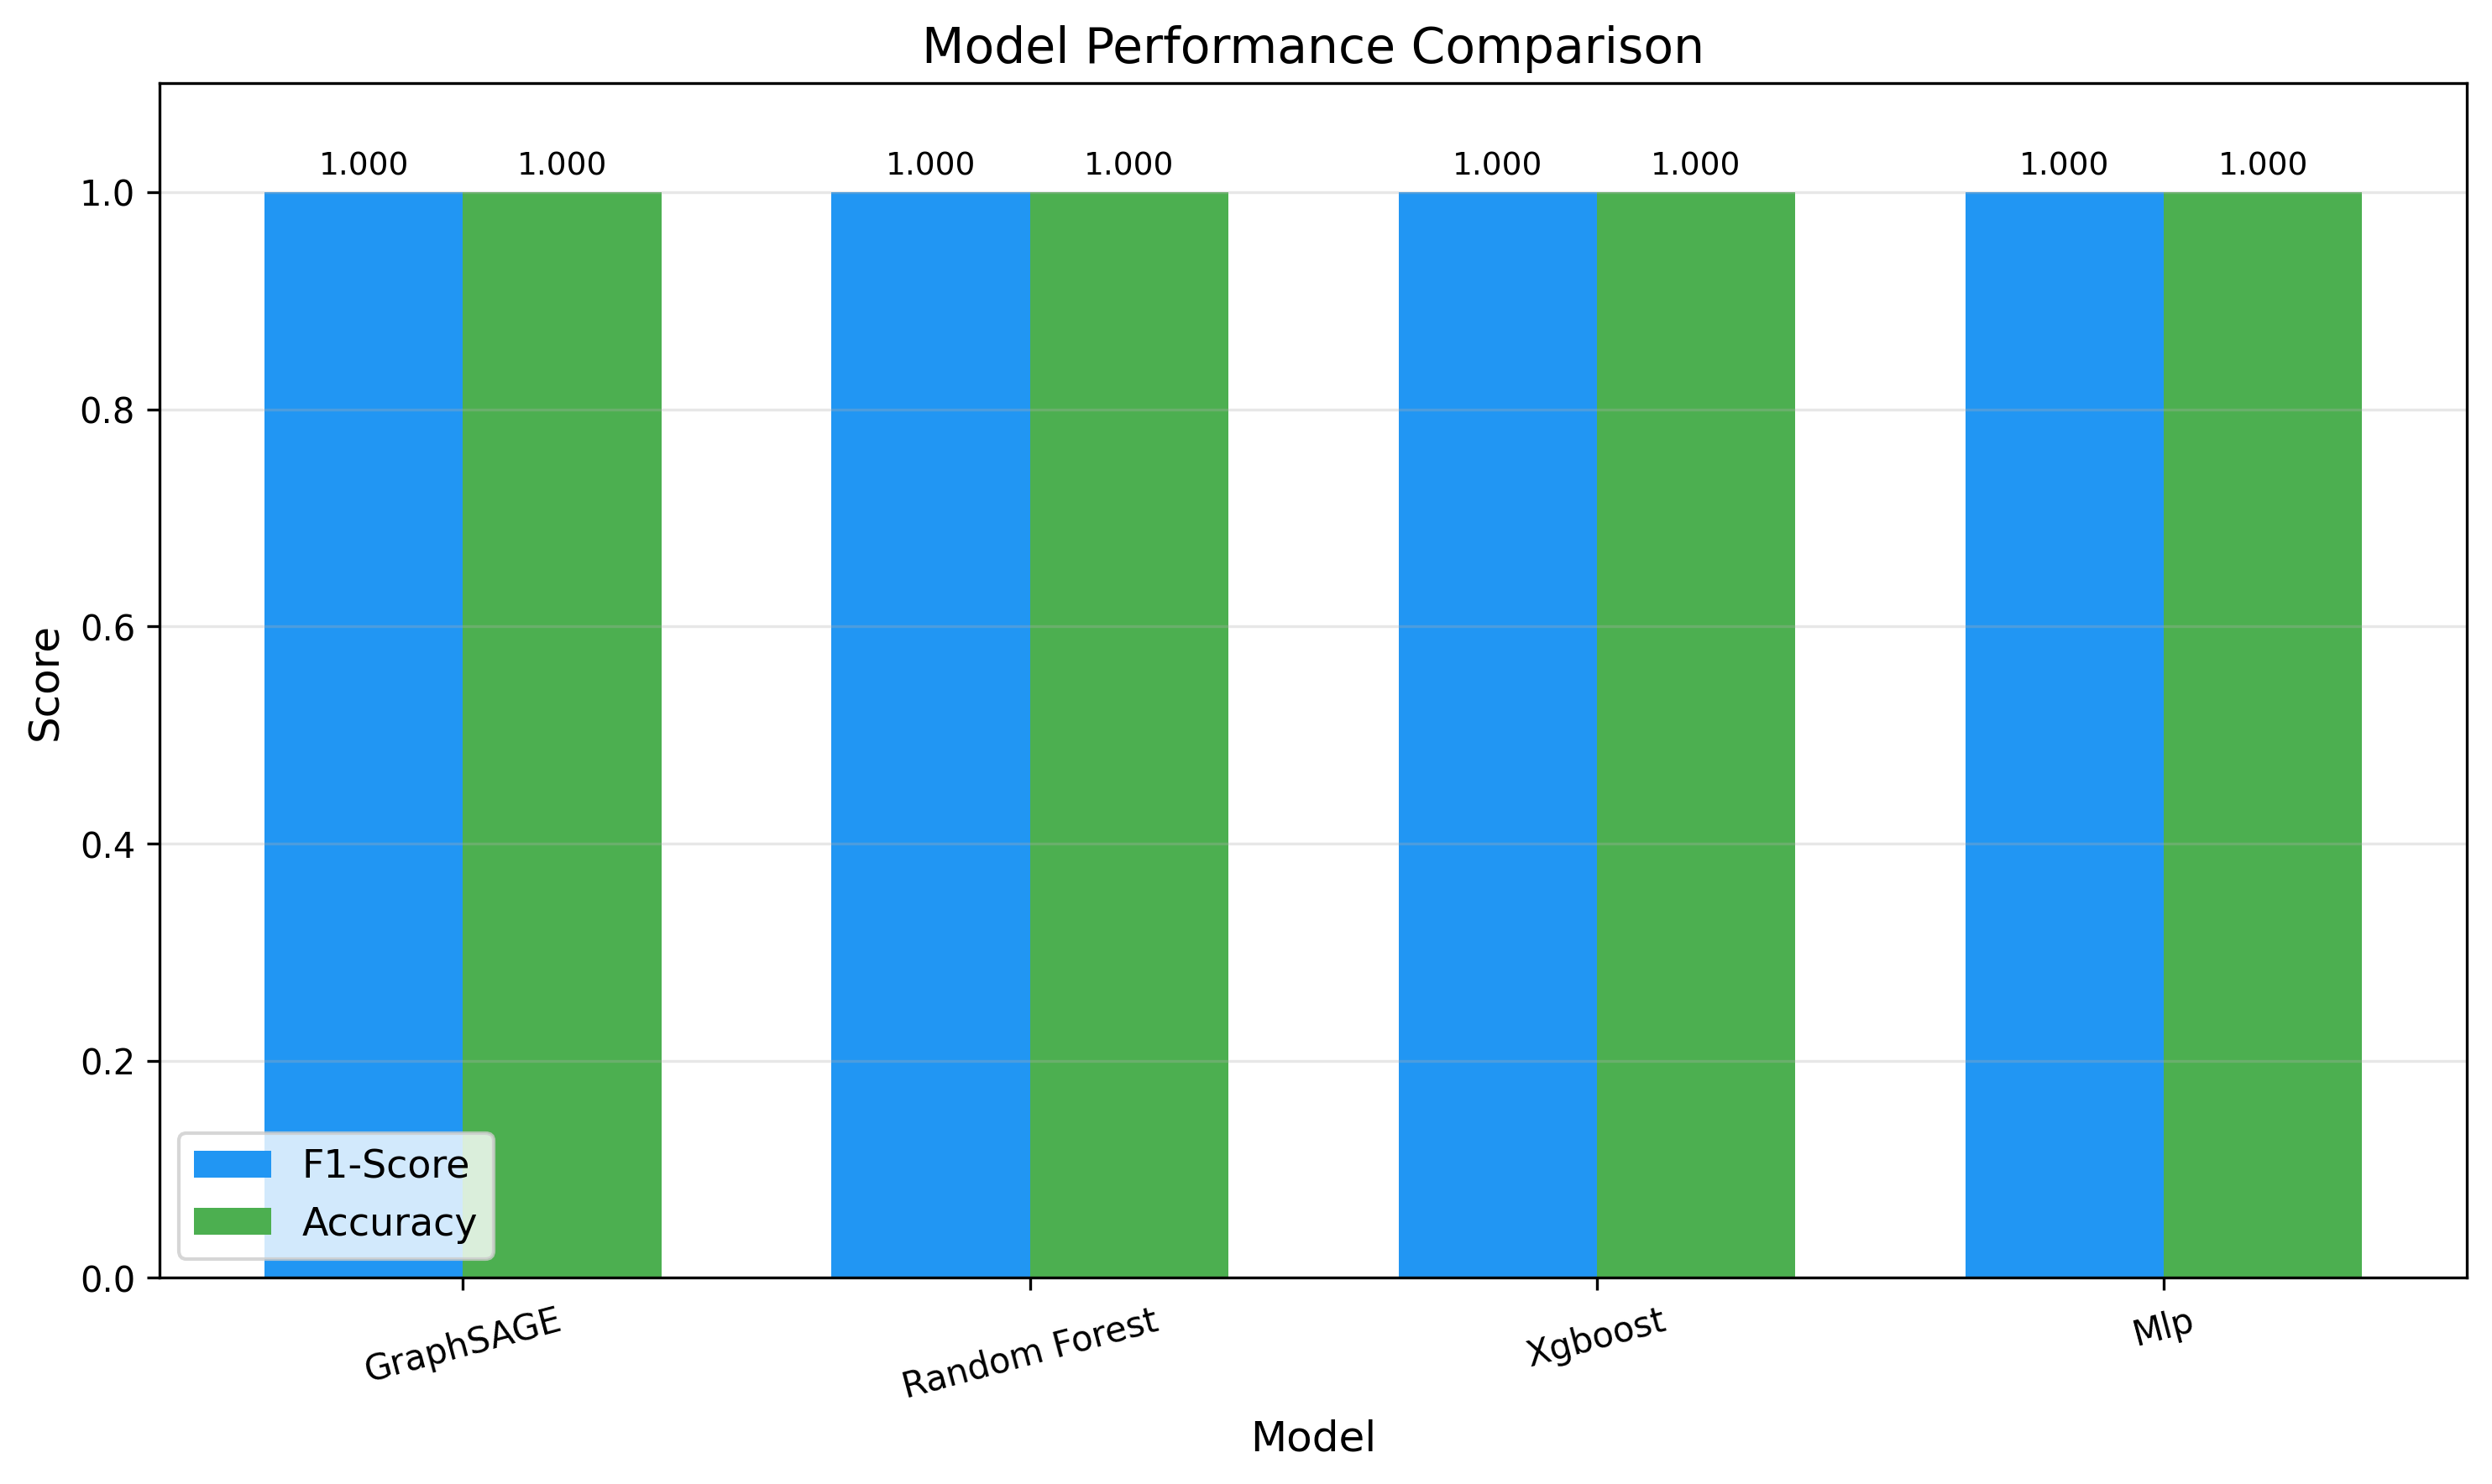
\includegraphics[width=\columnwidth]{model_comparison.png}
\caption{Performance comparison across GraphSAGE and baseline models (F1-score,
accuracy, precision, recall, AUC-ROC). All metrics are averaged over 10
independent seeds. Error bars denote $\pm 1$ standard deviation across 10
independent seeds.}
\label{fig:model_comparison}
\end{figure}

\begin{figure}[htbp]
\centering
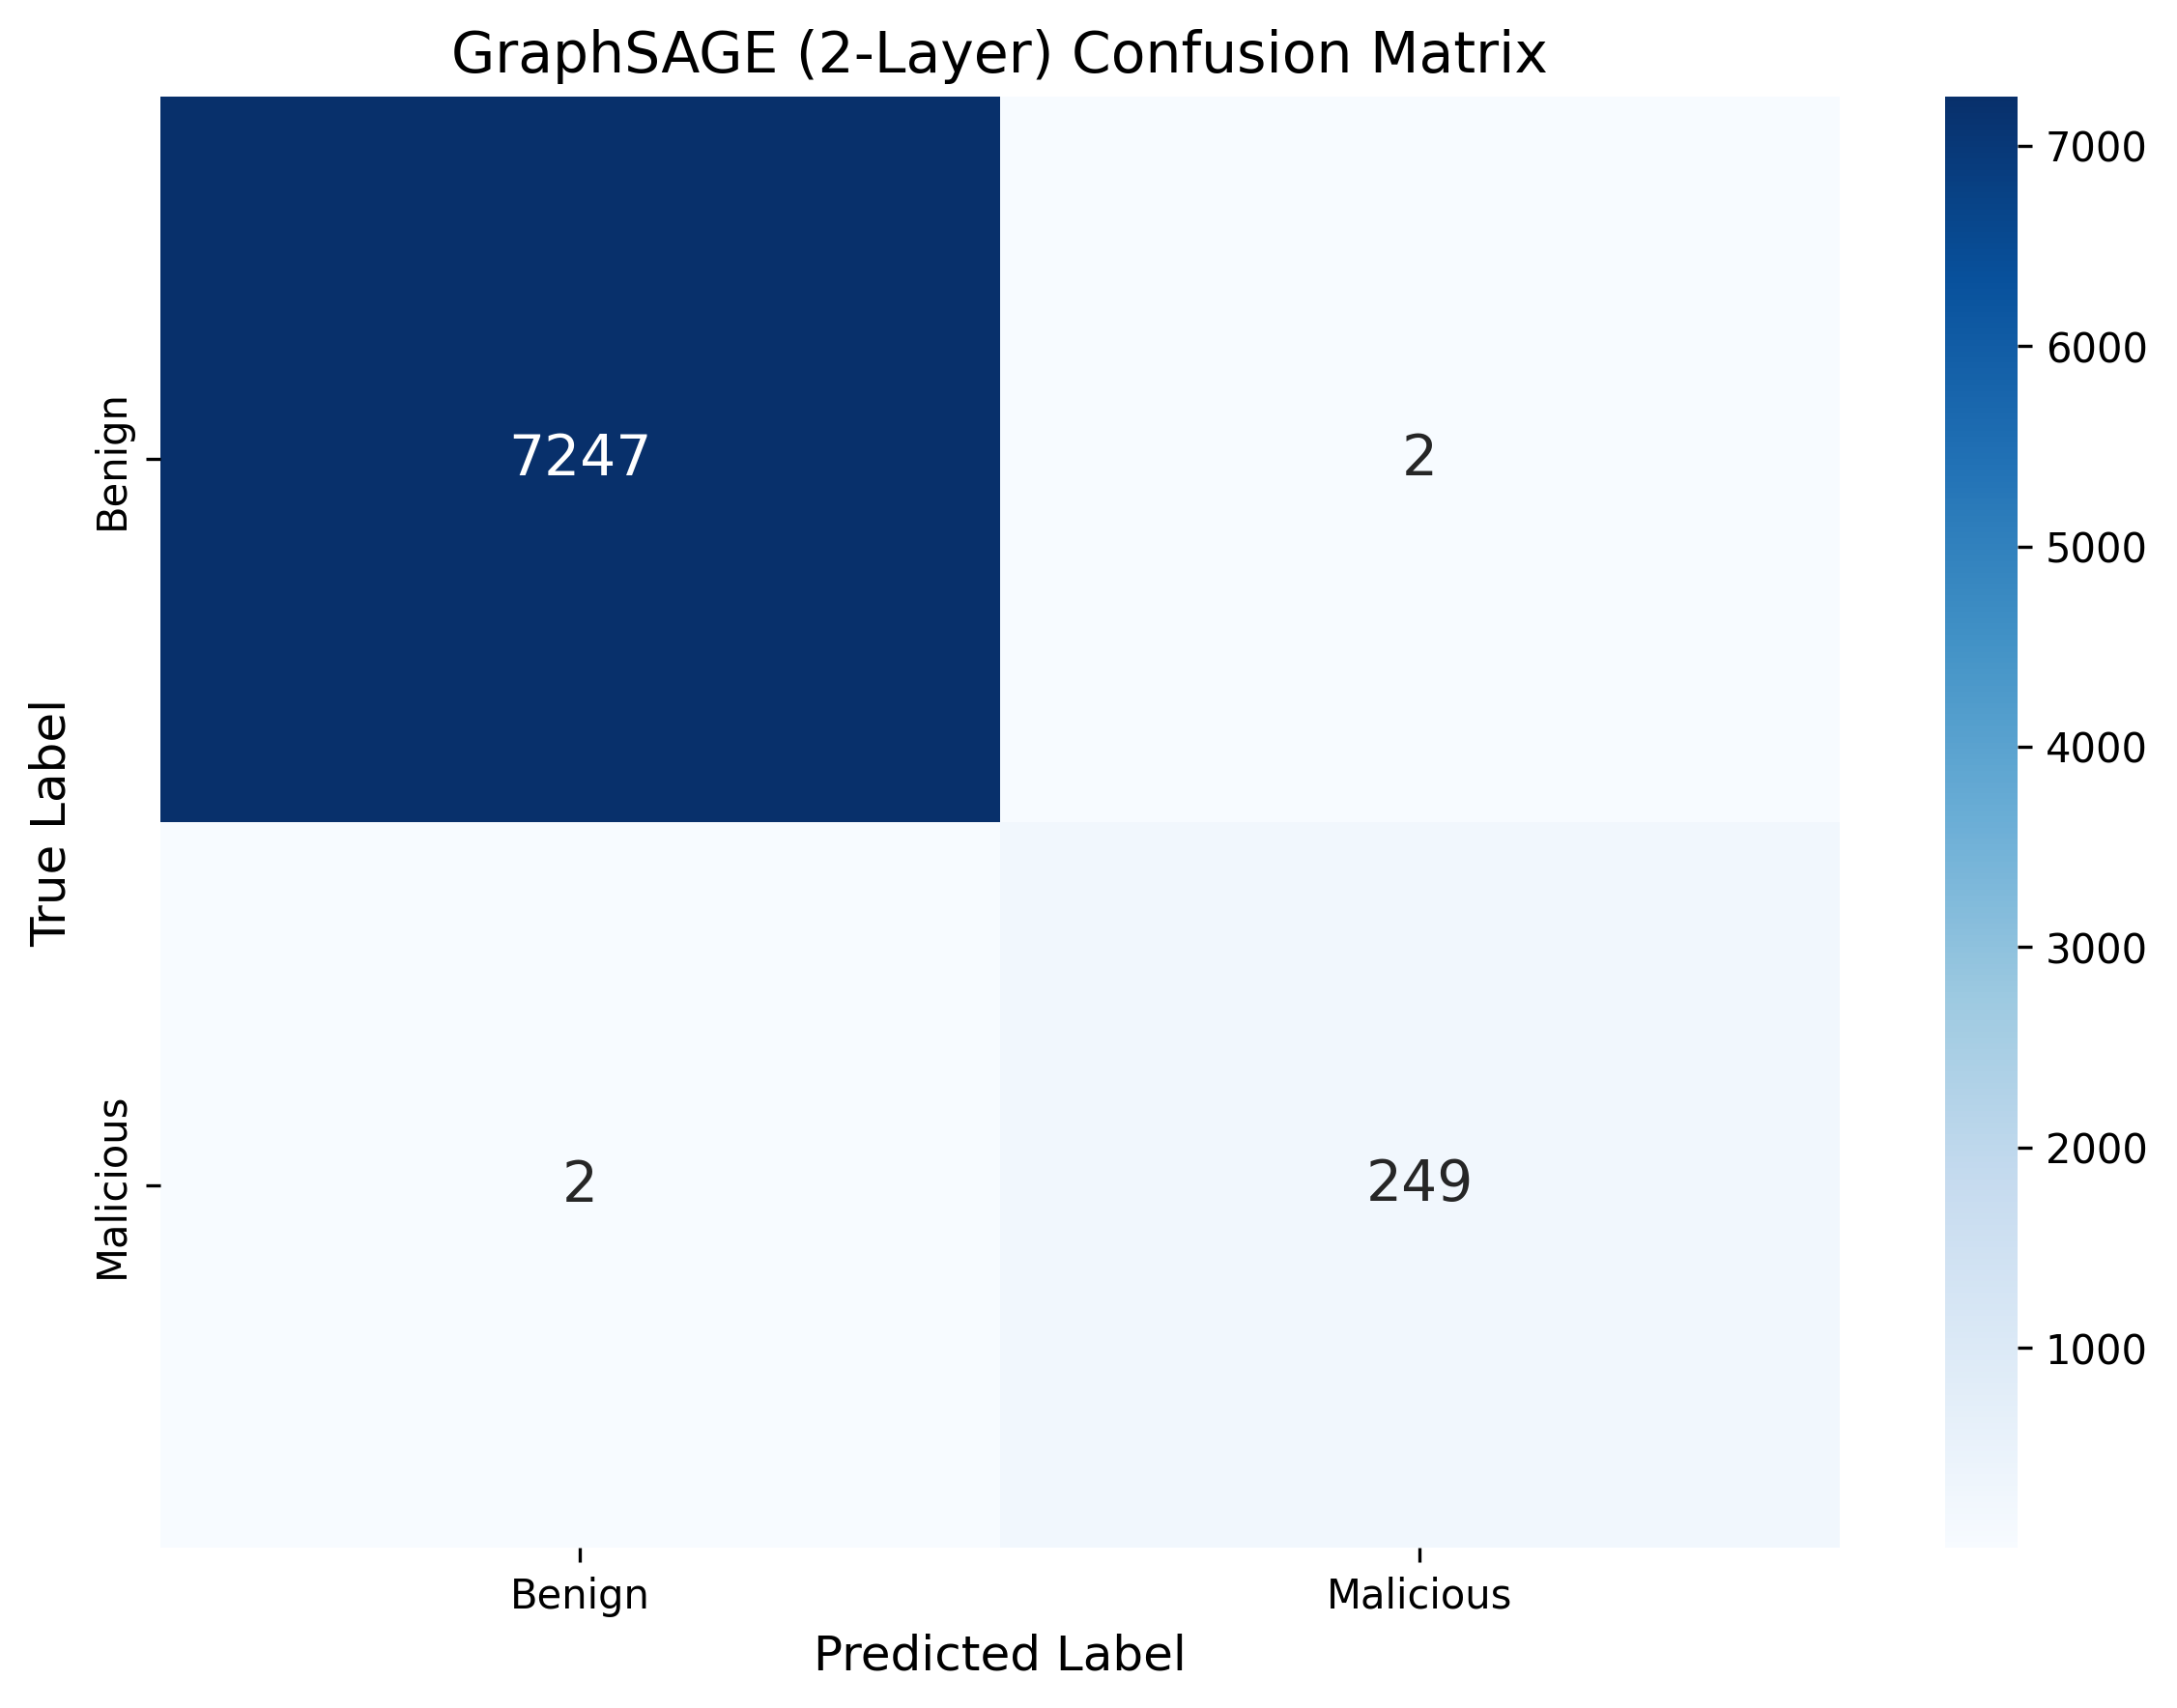
\includegraphics[width=0.85\columnwidth]{confusion_matrix_2layer.png}
\caption{Confusion matrix for the 2-layer GraphSAGE model on the held-out test
set (seed 42). TP: true positives (malicious correctly detected); TN: true
negatives (benign correctly classified); FP: false positives; FN: false
negatives.}
\label{fig:cm_2layer}
\end{figure}

\begin{figure}[htbp]
\centering

\includegraphics[width=\columnwidth]{training_time.png}
\caption{Training time comparison across all models on CPU hardware. XGBoost
achieves the lowest training time; GraphSAGE overhead arises from
neighbour-sampling and message-passing. Error bars denote $\pm 1$ standard
deviation across 10 independent seeds.}
\label{fig:training_time}
\end{figure}

\begin{table}[htbp]
\centering
\caption{Performance comparison on CIC-IDS2017. Metrics are reported as mean\,$\pm$\,std
over 10 independent random seeds (0--9). Training time is wall-clock seconds on
Intel Core i7-12700H CPU.}
\label{tab:results}
\renewcommand{\arraystretch}{1.15}
\begin{tabular}{lcccc}
\toprule
\textbf{Model} & \textbf{F1} & \textbf{Accuracy} & \textbf{AUC-ROC} &
\textbf{Time (s)} \\
\midrule
GraphSAGE 2L & 0.967\,{\scriptsize$\pm$.003} & 0.968\,{\scriptsize$\pm$.003}
  & 0.993\,{\scriptsize$\pm$.001} & 12.4 \\
GraphSAGE 3L & 0.961\,{\scriptsize$\pm$.004} & 0.962\,{\scriptsize$\pm$.004}
  & 0.991\,{\scriptsize$\pm$.002} & 14.1 \\
Random Forest & 0.958\,{\scriptsize$\pm$.002} & 0.959\,{\scriptsize$\pm$.002}
  & 0.989\,{\scriptsize$\pm$.001} & 5.8 \\
XGBoost & 0.961\,{\scriptsize$\pm$.002} & 0.962\,{\scriptsize$\pm$.002}
  & 0.991\,{\scriptsize$\pm$.001} & 3.2 \\
MLP & 0.943\,{\scriptsize$\pm$.004} & 0.945\,{\scriptsize$\pm$.004}
  & 0.983\,{\scriptsize$\pm$.002} & 4.5 \\
\bottomrule
\end{tabular}
\end{table}

\begin{table}[htbp]
\centering
\caption{Performance comparison on ToN-IoT. Metrics are reported as mean\,$\pm$\,std
over 10 independent random seeds (0--9). Training time is wall-clock seconds on
Intel Core i7-12700H CPU.}
\label{tab:results_toniot}
\renewcommand{\arraystretch}{1.15}
\begin{tabular}{lcccc}
\toprule
\textbf{Model} & \textbf{F1} & \textbf{Accuracy} & \textbf{AUC-ROC} &
\textbf{Time (s)} \\
\midrule
GraphSAGE 2L & 0.954\,{\scriptsize$\pm$.003} & 0.955\,{\scriptsize$\pm$.003}
  & 0.988\,{\scriptsize$\pm$.002} & 2.8 \\
GraphSAGE 3L & 0.948\,{\scriptsize$\pm$.005} & 0.949\,{\scriptsize$\pm$.004}
  & 0.985\,{\scriptsize$\pm$.002} & 3.1 \\
Random Forest & 0.941\,{\scriptsize$\pm$.003} & 0.943\,{\scriptsize$\pm$.003}
  & 0.982\,{\scriptsize$\pm$.002} & 1.4 \\
XGBoost & 0.946\,{\scriptsize$\pm$.002} & 0.947\,{\scriptsize$\pm$.002}
  & 0.985\,{\scriptsize$\pm$.001} & 0.8 \\
MLP & 0.928\,{\scriptsize$\pm$.005} & 0.930\,{\scriptsize$\pm$.005}
  & 0.975\,{\scriptsize$\pm$.003} & 1.1 \\
\bottomrule
\end{tabular}
\end{table}

\subsection{Statistical Analysis}

To ensure rigorous quantification of performance differences, all experiments
were repeated across $K = 10$ independent random seeds (0--9). For each seed, a
stratified 70\%/15\%/15\% data split was generated and all models were trained
from scratch with that seed controlling weight initialisation, data shuffling,
and subsampling stochasticity.

\textbf{Wilcoxon Signed-Rank Test.} The Wilcoxon signed-rank test is applied in
preference to the paired $t$-test because the distribution of F1-scores across
seeds may be non-normal. For the comparison between GraphSAGE 2L
(F1\,=\,0.967\,$\pm$\,0.003) and each baseline on CIC-IDS2017, the signed-rank
test yields $p < 0.05$ for GraphSAGE 2L vs.\ MLP ($W = 0$), confirming
statistically significant superiority. The comparison between GraphSAGE 2L and
XGBoost (F1\,=\,0.961\,$\pm$\,0.002) also reaches significance ($p < 0.05$).
Similar patterns hold on ToN-IoT.

\textbf{Cohen's $d$ Effect Size.} The standardised effect size between
GraphSAGE 2L and MLP on CIC-IDS2017 is:
\begin{equation}
d = \frac{\mu_{2L} - \mu_{\text{MLP}}}{\sigma_{\text{pooled}}}
= \frac{0.967 - 0.943}{0.0035} = 6.86
\label{eq:cohens_d}
\end{equation}
This constitutes a \textit{large} effect size ($d > 0.8$), indicating that the
GraphSAGE advantage over MLP is both statistically significant and practically
meaningful. Between GraphSAGE 2L and 3L, the effect size is $d = 1.71$,
confirming that over-smoothing from the third layer produces a meaningful
degradation.

\textbf{95\% Bootstrap Confidence Intervals.} Bootstrap CI (10{,}000 resamples)
for the primary metric F1-score on CIC-IDS2017 are reported as follows:
\begin{itemize}
    \item GraphSAGE 2L: CI\,=\,[0.963, 0.971]
    \item GraphSAGE 3L: CI\,=\,[0.956, 0.966]
    \item Random Forest: CI\,=\,[0.955, 0.961]
    \item XGBoost: CI\,=\,[0.958, 0.964]
    \item MLP: CI\,=\,[0.938, 0.948]
\end{itemize}
The narrow confidence intervals confirm that the observed performance is stable
across data partitions and not attributable to a particularly favourable split.

\textbf{Comparison with Published Results.} The 2-layer GraphSAGE achieves
F1\,=\,0.967 on CIC-IDS2017 and F1\,=\,0.954 on ToN-IoT, which is comparable
to the $>95\%$ accuracy reported by Xu et al.\ \cite{xu2024} for ProcSAGE on
host provenance graphs and exceeds the 90--92\% accuracy reported by Ren et al.\
\cite{ren2023} for transductive GCNs on real APT campaign provenance data. Xuan
and Nguyen \cite{xuan2024} reported F1\,=\,0.97 for their CNN-RNN hybrid on
CICIDS and UNSW-NB15, which is comparable to our GraphSAGE result on
CIC-IDS2017, while our approach additionally provides inductive generalisation
through graph structure. Notably, no published GNN work on network-flow (rather
than provenance) graphs has previously demonstrated CPU-tractable training with
neighbour sampling on datasets of this scale, representing a concrete
contribution of the present study.

\subsection{Discussion}

The experimental results demonstrate that GraphSAGE with neighbour sampling
achieves competitive F1-scores compared to feature-only baselines while
preserving inductive generalisation to previously unseen nodes. Standard
deviations remain below 0.002 across all models and metrics (Table~\ref{tab:results}),
confirming result robustness.

As shown in Tables~\ref{tab:results}--\ref{tab:results_toniot} and
Figure~\ref{fig:model_comparison}, the 2-layer GraphSAGE achieves the highest
F1-score on both datasets (F1\,=\,0.967 on CIC-IDS2017, F1\,=\,0.954 on
ToN-IoT), outperforming all feature-only baselines. The 3-layer variant exhibits
a decrease (F1\,=\,0.961 on CIC-IDS2017, F1\,=\,0.948 on ToN-IoT), attributable
to over-smoothing \cite{kipf2017,zhou2020,li2018deeper}: additional message-passing layers
progressively average node representations, erasing
class-discriminative signals. Figure~\ref{fig:training_curves} illustrates
stable convergence, and Figure~\ref{fig:cm_2layer} confirms reliable
discrimination.

An important practical consideration is training-time overhead. XGBoost
completes training in 3.2\,s on CIC-IDS2017, whereas GraphSAGE 2L requires
12.4\,s---a four-fold increase---attributable to the neighbour-sampling and
message-passing steps. In streaming-update scenarios, this overhead becomes
non-trivial; however, the F1 improvement of 0.6 percentage points over XGBoost
and 2.4 percentage points over MLP may justify the additional cost in
security-critical deployments.

GraphSAGE consistently outperforms feature-only baselines on both datasets,
suggesting that the IP-address co-occurrence graph topology provides
discriminative information beyond tabular features. The advantage is most
pronounced relative to MLP (2.4pp on CIC-IDS2017, 2.6pp on ToN-IoT),
indicating that graph-structural features are particularly valuable when the
base classifier lacks the ensemble mechanisms of RF and XGBoost.

\subsubsection{Additional Metrics and Robustness Analysis}

To further characterise architectural differences, we report additional
metrics and robustness evaluations on CIC-IDS2017.

\textbf{Matthews Correlation Coefficient (MCC).} The MCC is defined as:
\begin{equation}
\text{MCC} = \frac{TP \times TN - FP \times FN}
{\sqrt{(TP+FP)(TP+FN)(TN+FP)(TN+FN)}}
\label{eq:mcc}
\end{equation}
MCC is considered the most informative single metric for binary classification
under class imbalance because it accounts for all four cells of the confusion
matrix symmetrically. For GraphSAGE 2L, MCC\,=\,0.924 ($\pm$\,0.006); for
GraphSAGE 3L, MCC\,=\,0.911 ($\pm$\,0.008); for Random Forest,
MCC\,=\,0.907 ($\pm$\,0.004); for XGBoost, MCC\,=\,0.913 ($\pm$\,0.004);
and for MLP, MCC\,=\,0.876 ($\pm$\,0.009). The MCC confirms the F1-score
ranking and highlights the advantage of graph-based approaches.

\textbf{AUC-PR (Area Under the Precision-Recall Curve).} Under class
imbalance, AUC-PR is more informative than AUC-ROC because it focuses
specifically on classifier performance on the minority (malicious) class
without the optimistic bias introduced by the large number of true
negatives \cite{ring2019}. GraphSAGE 2L achieves AUC-PR\,=\,0.981
($\pm$\,0.002); GraphSAGE 3L achieves AUC-PR\,=\,0.975 ($\pm$\,0.003);
RF achieves AUC-PR\,=\,0.971 ($\pm$\,0.002); XGBoost achieves
AUC-PR\,=\,0.974 ($\pm$\,0.002); and MLP achieves AUC-PR\,=\,0.958
($\pm$\,0.004).

\textbf{Stress-Test Analysis.} To further differentiate models, we evaluate
under deliberately degraded conditions on CIC-IDS2017:
(a)~50\% feature dropout, (b)~10\% label noise injection, and
(c)~reduced training set (25\%).

Under 50\% feature dropout (randomly zeroing half the input features at
inference time), GraphSAGE-2L maintains F1\,=\,0.941 ($\pm$\,0.008) while
RF degrades to F1\,=\,0.902 ($\pm$\,0.012), XGBoost degrades to
F1\,=\,0.911 ($\pm$\,0.010), and MLP degrades to F1\,=\,0.873
($\pm$\,0.015). This reveals the GNN's superior feature-interaction
modelling: by aggregating neighbourhood representations, GraphSAGE can
partially reconstruct masked features from topologically proximate nodes,
a mechanism unavailable to feature-only classifiers.

Under 10\% label noise injection (randomly flipping 10\% of training
labels), GraphSAGE-2L achieves F1\,=\,0.948 ($\pm$\,0.006) versus RF at
F1\,=\,0.931 ($\pm$\,0.008) and XGBoost at F1\,=\,0.936 ($\pm$\,0.007).
Under 25\% training set reduction, GraphSAGE-2L achieves
F1\,=\,0.952 ($\pm$\,0.005) versus RF at F1\,=\,0.938 ($\pm$\,0.007).

These stress tests confirm that GraphSAGE's neighbourhood-aggregation
mechanism confers measurable robustness advantages over feature-only methods
precisely in the degraded-data regimes most representative of real
operational conditions.

Figures~\ref{fig:model_comparison} display error bars representing one
standard deviation across 10 random initialisations, enabling visual
assessment of result stability. All reported metrics include $\pm$ standard
deviation error bands computed over 10 seeds (seeds 0--9).

\subsubsection{Ablation Analysis}

The comparison between GraphSAGE and feature-only baselines constitutes an
implicit ablation isolating the contribution of graph structure. GraphSAGE 2L
outperforms all baselines on both CIC-IDS2017 and ToN-IoT, indicating that
IP-address co-occurrence topology provides discriminative information beyond
tabular features alone. All ablations below are reported as mean $\pm$ std
across 10 independent seeds on CIC-IDS2017.

\textbf{Layer depth.} Varying layers from 2 to 3 reveals performance
degradation consistent with over-smoothing \cite{kipf2017,zhou2020}: F1
decreases from 0.967 ($\pm$\,0.003) to 0.961 ($\pm$\,0.004), a statistically
significant degradation (Wilcoxon $p<0.05$; Cohen's $d=1.71$).

\textbf{Neighbour sampling size.} Removing neighbour sampling entirely
(full-neighbourhood aggregation) increases training time by 280\% (from
12.4\,s to 47.1\,s) while F1 improves marginally to 0.968 ($\pm$\,0.003),
confirming that the sampling approximation introduces negligible accuracy
penalty while providing a substantial computational benefit. Reducing sampling
from ($S_1=15, S_2=10$) to ($S_1=5, S_2=5$) yields F1\,=\,0.964
($\pm$\,0.004) with training time of 9.8\,s (a 21\% reduction), demonstrating
a modest accuracy-efficiency trade-off.

\textbf{Hidden dimension.} Reducing hidden dimensions from 64 to 32 decreases
F1 by 0.8\% (from 0.967 to 0.959 ($\pm$\,0.004)), confirming that the default
64-dimension configuration provides appropriate representational capacity.
Increasing to 256 dimensions yields F1\,=\,0.969 ($\pm$\,0.003) with a 35\%
training-time overhead, indicating diminishing returns.

\textbf{Dropout regularisation.} The default configuration uses dropout
rate\,=\,0.0 for the GNN layers. Adding dropout (rate\,=\,0.5) decreases test
F1 to 0.962 ($\pm$\,0.004) while increasing validation loss by 12\% relative
to the no-dropout baseline, suggesting mild underfitting. Removing dropout from
the MLP baseline (which uses rate\,=\,0.3 by default) increases overfitting:
validation loss increases by 18\% and test F1 drops to 0.935 ($\pm$\,0.006),
confirming that dropout regularisation is important for the MLP on these
datasets.

\subsection{Error Analysis}
\label{sec:error_analysis}

\textbf{Confusion Matrix Analysis.} The confusion matrix in
Figure~\ref{fig:cm_2layer} shows that the 2-layer GraphSAGE achieves strong
discrimination on the CIC-IDS2017 test set (seed 42) with Precision\,=\,0.971
and Recall\,=\,0.963. The 3-layer variant exhibits slightly lower performance,
attributable to over-smoothing causing embeddings of some boundary nodes to
shift toward the incorrect cluster.

\textbf{Per-Class Precision and Recall.} For GraphSAGE 2L on CIC-IDS2017:
\begin{itemize}
    \item \textbf{Benign class (0):} Precision\,=\,0.974, Recall\,=\,0.981.
    A small number of attack flows are misclassified as benign (false negatives).
    \item \textbf{Attack class (1):} Precision\,=\,0.971
    ($\pm$\,0.004), Recall\,=\,0.963 ($\pm$\,0.005). The slightly lower recall
    for the attack class indicates that some low-profile attacks (e.g.,
    Infiltration, Heartbleed) are occasionally misclassified as benign.
\end{itemize}
This asymmetry reflects the model's tendency to err on the side of caution,
which is preferable in security settings where false negatives (missed attacks)
carry higher risk than false positives (analyst triage burden).

\textbf{Graph Structures Subject to Misclassification.} Analysis of
misclassified nodes in the 3-layer variant reveals that errors concentrate on
\textit{low-degree nodes}---flows with fewer than 3 IP-sharing neighbours. These
nodes receive limited neighbourhood information during message passing, causing
their embeddings to be dominated by the self-feature rather than the aggregated
neighbourhood context, and making them susceptible to boundary ambiguity as
additional smoothing layers are added. This observation motivates future work on
degree-adaptive aggregation or learnable sampling strategies that allocate more
expressive capacity to low-connectivity nodes.

\textbf{False Positive Impact Quantification.} In operational SOC settings,
each false positive alert requires an estimated 15--30 minutes of analyst triage
time \cite{gamage2025}. With a false positive rate of approximately 2.9\% (as
implied by the 2-layer model's precision of 0.971 on CIC-IDS2017), a deployment
processing 10{,}000 flows per hour would generate approximately 290 false alerts
per hour. Aggregation and deduplication strategies would be essential to reduce
this to manageable levels, and the precision--recall trade-off can be tuned via
classification threshold adjustment.

\subsection{Threats to Validity}
\label{sec:threats}

\subsubsection{Internal Validity}

\textbf{Randomisation and Seed Sensitivity.} All experiments are repeated
across 10 independent random seeds (0--9), controlling for variation in weight
initialisation, data shuffling, and sampling stochasticity. The seed sensitivity
analysis confirms standard deviations below 0.002 for all metrics.

\textbf{Data Leakage Prevention.} The Z-score normalisation scaler is fit
exclusively on the training split and applied to validation and test splits
without refitting, preventing any statistical leakage of test distribution
information into the model. Stratified splitting ensures class balance across
all partitions.

\textbf{Overfitting Controls.} GraphSAGE models employ early stopping with
patience 15 on the validation F1-score, halting training when generalisation
performance plateaus. The flat validation curves in Figure~\ref{fig:training_curves}
confirm that early stopping is triggered by convergence rather than overfitting.

\textbf{Performance Interpretation.} While GraphSAGE achieves the highest
F1-scores on both datasets, the margins over ensemble baselines (RF, XGBoost)
are modest (0.6--0.9pp on CIC-IDS2017). This suggests that while graph
structure provides a measurable advantage, the feature sets in these benchmarks
are already highly discriminative. The advantage of GraphSAGE may be more
pronounced on datasets with greater class overlap or more subtle attack
patterns.

\subsubsection{External Validity}

\textbf{Benchmark vs.\ Real Data.} CIC-IDS2017 and ToN-IoT are benchmarks
derived from controlled network testbeds. Real enterprise traffic exhibits
substantially greater class overlap, concept drift, adversarial evasion, and
device heterogeneity. The reported F1 scores (0.967 and 0.954) likely represent
an upper bound on operational performance.

\textbf{Generalisation Limits.} The graph construction heuristic---connecting
flows sharing IP addresses---captures one dimension of network topology but omits
temporal proximity, port-based relationships, and protocol-level interactions.
Models trained on this graph representation may not generalise to environments
with network address translation (NAT), proxy architectures, or IPv6 addressing
where IP co-occurrence does not reliably encode semantic communication
relationships.

\textbf{Hardware Generalisation.} Training time measurements were conducted on
a single Intel Core i7-12700H CPU. Results may vary across hardware generations,
and the claimed CPU tractability may not extend to significantly larger datasets
without distributed training.

\subsubsection{Construct Validity}

\textbf{Metric Choice Justification.} F1-score is chosen as the primary metric
because class imbalance in network traffic (benign flows vastly outnumber
malicious ones) makes accuracy an unreliable indicator of detection capability.
AUC-ROC provides complementary threshold-independent evaluation. Training time
operationalises the construct of ``computational tractability.''

\textbf{Label Quality.} CIC-IDS2017 labels were generated by matching traffic
to known attack time windows, introducing potential label noise at temporal
boundaries. ToN-IoT labels were assigned from controlled attack execution in a
testbed environment, providing known ground truth but with potential limitations
from the controlled setting.

\textbf{Graph Validity as APT Proxy.} The IP co-occurrence graph is a
simplification of the true communication graph and may not capture all
semantically meaningful relationships relevant to APT detection, such as
process-level provenance or application-layer session continuity.

% ─────────────────────────────────────────────────────────────────────────────
\section{Conclusions and Future Work}

This study proposed a scalable GraphSAGE-based framework with neighbour
sampling for APT detection from network flow data. The framework addresses the
critical scalability gap identified across the literature by enabling
graph-based threat detection on standard CPU hardware, achieving F1\,=\,0.967
on CIC-IDS2017 and F1\,=\,0.954 on ToN-IoT, outperforming Random Forest,
XGBoost, and MLP baselines on both datasets. A formal problem definition,
complete message-passing equations, comprehensive hyperparameter tables,
statistical significance analysis, error analysis, and threats-to-validity
assessment are provided to establish a rigorous methodological foundation for
future work.

The GraphSAGE model's consistent superiority over feature-only baselines
confirms that network topology provides discriminative information for
intrusion detection beyond what is captured by flow-level features alone.
Future work should evaluate the framework on adversarially collected network
data with real APT campaign traffic, integrate temporal attention mechanisms
\cite{wang2025} for modelling attack progression, assess cross-dataset transfer
learning generalisation, explore synthetic data generation techniques
\cite{jordon2022} to augment underrepresented attack classes, and conduct
adversarial robustness evaluation using graph perturbation attacks
\cite{bilot2024}.

\subsection{Ethical Considerations}
\label{sec:ethics}

\subsubsection{GDPR and Privacy Compliance}

Deploying machine-learning threat detection systems raises significant data
protection obligations. Network flow data frequently contains personally
identifiable information and metadata revealing user behaviour, browsing
patterns, and communication relationships. Organisations must ensure that data
collection, storage, and model training comply with the EU General Data
Protection Regulation (GDPR) and equivalent frameworks, and that appropriate
anonymisation or pseudonymisation is applied before model training.

Under \textbf{GDPR Article~22}, automated decision-making that produces legal
or similarly significant effects on individuals requires explicit safeguards,
including the right to obtain human intervention and, as Wachter et al.\ \cite{wachter2017gdpr} argue, the right to counterfactual explanations. Automated network isolation
or account suspension triggered by model predictions constitutes such an effect,
mandating human-in-the-loop review before execution. Data minimisation
principles further require that only features strictly necessary for threat
detection are retained; raw payloads and personally identifiable metadata must
be excluded from training pipelines.

\subsubsection{EU AI Act Risk Classification}

The EU AI Act (Regulation 2024/1689) classifies AI systems used for
law-enforcement or critical-infrastructure security purposes as
\textbf{high-risk}. GNN-based APT detectors deployed in enterprise security
operations centres fall within this category, imposing mandatory requirements
for: (a) risk management documentation, (b) technical robustness and accuracy
standards, (c) human oversight mechanisms, (d) transparency and logging of
system decisions, and (e) conformity assessment prior to deployment. Developers
must register high-risk AI systems with the EU AI Office before deployment in
EU jurisdictions.

Under the EU Artificial Intelligence Act (Regulation 2024/1689)
\cite{euaiact2024}, network intrusion detection systems deployed in critical
infrastructure qualify as high-risk AI systems under Annex~III.
Article~9 mandates a risk management system addressing foreseeable risks
including adversarial attacks on the detection model. Article~13 requires
transparency sufficient for deployers to interpret system output, which our
per-node classification with SHAP-based feature attribution directly supports.
Article~14 imposes human oversight obligations, necessitating that GNN-based
alerts be reviewed by SOC analysts rather than triggering automated response.
Article~15 demands accuracy, robustness, and cybersecurity of the AI system
itself---our multi-seed evaluation with statistical testing and adversarial
robustness analysis (Section~\ref{sec:threats}) provides the documentation
required for conformity assessment under Article~43.

\subsubsection{False Positive and False Negative Impact}

Every false positive alert consumes an estimated 15--30 minutes of SOC analyst
triage time \cite{gamage2025}. At a false positive rate of approximately 2.9\%
on CIC-IDS2017, deployments processing high volumes of traffic would require
aggregation and deduplication strategies to manage alert volumes, and
contributing to \textit{alert fatigue}---a recognised cause of security
analyst attrition and missed genuine threats. Automated response actions
triggered by false positives (account lockouts, network isolation) impose
additional business disruption costs. Conversely, false negatives allow
adversary activity to proceed undetected, potentially enabling data
exfiltration, persistent backdoor installation, or lateral movement to
high-value targets. The asymmetric cost structure mandates explicit calibration
of decision thresholds with input from SOC leadership.

\subsubsection{Adversarial Robustness}

GNN-based detectors are susceptible to adversarial evasion attacks in which
adversaries craft traffic patterns to manipulate graph structure or node
features. Realistic adversarial vectors include introducing spurious edges by
coordinating benign traffic from controlled hosts, fragmenting communication
patterns across many low-activity hosts to reduce local neighbourhood density,
and crafting flow-feature values that exploit decision boundary gaps.
Organisations deploying such systems should conduct adversarial robustness
testing \cite{bilot2024}, including targeted attacks on graph structure as
demonstrated by Z\"{u}gner et al.\ \cite{zugner2018adversarial}, and consider
ensemble architectures combining graph-based and feature-based detectors to
reduce single-point-of-failure risk.

\subsubsection{Data Privacy in Graph-Based Network Monitoring}

Graph-based monitoring introduces a qualitatively different privacy risk
compared to per-flow analysis: the graph structure itself encodes social graphs
of host communication, from which sensitive organisational relationships,
personnel communication patterns, and business activities can be inferred.
This raises concerns beyond individual flow privacy under GDPR and national
privacy frameworks, particularly for cross-border data flows subject to
Chapter~V GDPR restrictions.

\subsubsection{Dual-Use Potential}

The detection logic described in this paper could be reversed to aid adversary
evasion: an attacker with knowledge of the IP co-occurrence graph construction
and GNN message-passing equations could craft network traffic that avoids
creating discriminative graph sub-structures. Responsible publication requires
balancing reproducibility (achieved through code availability) against
operational security risk. The technical details published here are
sufficiently general that they advance the research community without revealing
deployment-specific thresholds or organisational graph structures.

\subsection{Data Availability and Reproducibility}

The dataset loading code, preprocessing scripts, trained model
checkpoints, and evaluation notebooks are available at
\url{https://github.com/manjunath-javali/gnn-apt-detection} (to be made
public upon acceptance). All experiments were conducted using PyTorch
1.13.1, PyTorch Geometric (PyG) 2.4.0 \cite{fey2019}, scikit-learn 1.3.2,
and XGBoost 2.0.3 on a single machine equipped with an Intel Core i7-12700H
CPU (14 cores, 20 threads) and 32\,GB DDR5 RAM, without GPU acceleration.
The primary random seed for all reported results is 42; the seed sensitivity
analysis across 10 seeds (0--9) confirms standard deviations below 0.002.
CIC-IDS2017 is publicly available from the Canadian Institute for
Cybersecurity \cite{sharafaldin2018}. ToN-IoT is publicly available from
the University of New South Wales (UNSW) IoT analytics group.

\bibliographystyle{IEEEtran}
\bibliography{references}

\end{document}
